\documentclass[12pt]{article}
\usepackage{graphicx}
\usepackage{fancyhdr}
\usepackage{varwidth}
\usepackage{commath}
\usepackage{xspace}
\begin{document}
\begin{center}

\pagestyle{fancy}
\lhead{Steven Seiden}
\rhead{The ``Ultimate" 1022 Math Formula Sheet}



\large
Special Right Triangles\\
\\~\\
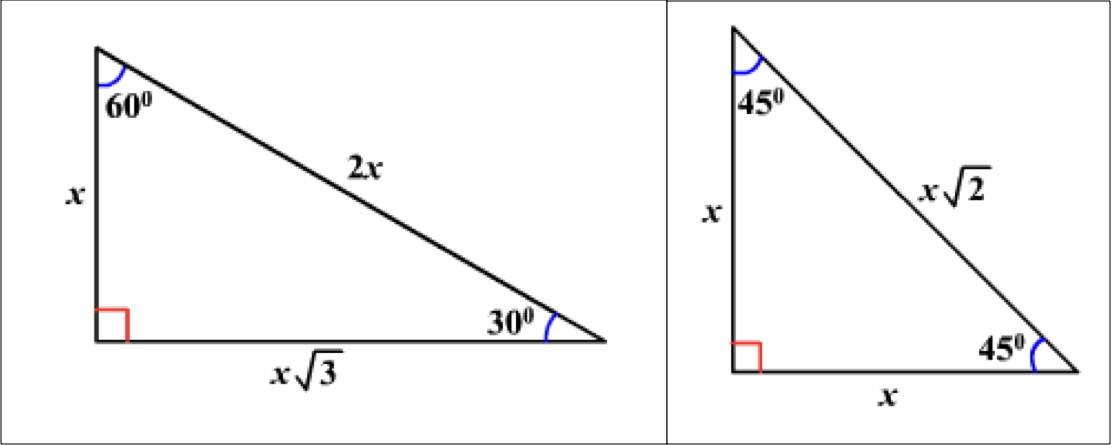
\includegraphics[width=100mm,scale=0.5]{Triangles.png}}\\


\\[.75in]
\large
Converting between radians and degrees\\
\normalsize
\\~\\
radians = \left( {\pi }\over {180^{\circ }}\right) \cdot degrees\\~\\
degrees = \left( {180^{\circ }}\over {\pi}\right) \cdot radians



\\[.75in]
\large
The Unit Circle + hand trick
\normalsize
\\~\\
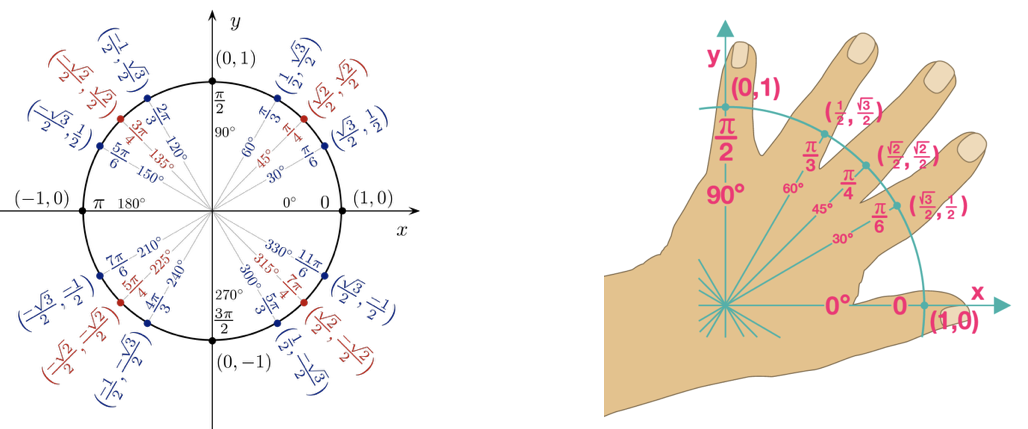
\includegraphics[width=150mm,scale=0.5]{unitcircle.png}}


\\[.75in]
\large
Definitions of sine, cosine, tangent and their reciprocals

\normalsize
\\~\\
\sin \theta ={{opposite}\over{hypotenuse}} \hspace{10mm}
\csc \theta ={{hypotenuse}\over{opposite}}
\\~\\
\cos \theta ={{adjacent}\over{hypotenuse}} \hspace{10mm}
\sec \theta ={{hypotenuse}\over{adjacent}}
\\~\\
\tan \theta ={{opposite}\over{adjacent}} \hspace{10mm}
\cot \theta ={{adjacent}\over{opposite}}




\\[.75in]
\large
Using sine, cosine and tangent with the unit circle

\normalsize
\\~\\
\sin \theta ={{y}\over{r}} \hspace{10mm}
\csc \theta ={{r}\over{y}}
\\~\\
\cos \theta ={{x}\over{r}} \hspace{10mm}
\sec \theta ={{r}\over{x}}
\\~\\
\tan \theta ={{y}\over{x}} \hspace{10mm}
\cot \theta ={{x}\over{y}}
\\~\\
x^2+y^2=r^2



\\[.75in]
\large
Simplifying trigonometric expressions (sine and cosine)
\normalsize
\\~\\
\sin(\alpha+\beta) = \sin \alpha \cos \beta + \cos \alpha \sin \beta\\
\cos(\alpha+\beta) = \cos \alpha \cos \beta - \sin \alpha \sin \beta\\
\sin(\alpha-\beta) = \sin \alpha \cos \beta - \cos \alpha \sin \beta\\
\cos(\alpha-\beta) = \cos \alpha \cos \beta + \sin \alpha \sin \beta\\



\newpage
\large
Arc length, sector area, and radius formulas
\normalsize
\\~\\

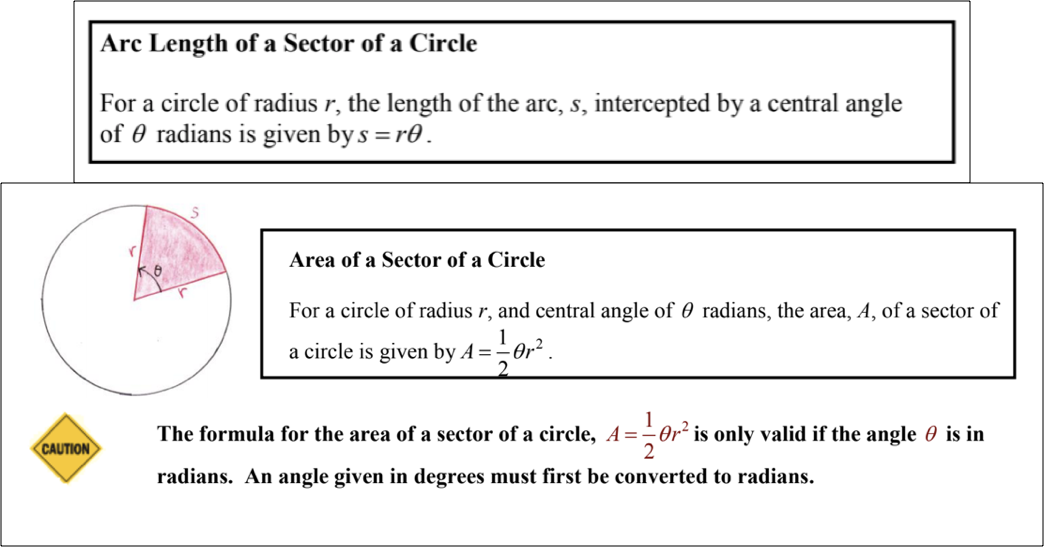
\includegraphics[width=125mm,scale=0.5]{arclen.png}}



\\[.75in]
\large
Trigonometric identities
\normalsize
\\~\\
\fbox{\parbox{\dimexpr\linewidth-2\fboxsep-2\fboxrule\relax}{\centering \textbf{Reciprocal Identities}  \\ 
	\\~\\
	\cot \theta = {{1}\over{\tan\theta}}
	\hspace{10mm}
	\sec \theta = {{1}\over{\cos\theta}}
	\hspace{10mm}
	\csc \theta = {{1}\over{\sin\theta}}\\~\\

}}%



\fbox{\parbox{\dimexpr\linewidth-2\fboxsep-2\fboxrule\relax}{\centering \textbf{Quotient Identities}  \\ 
	\\~\\
	\tan \theta = {{\sin\theta}\over{\cos\theta}}
	\hspace{10mm}
	\cot \theta = {{\cos\theta}\over{\sin\theta}}\\~\\

}}%

\fbox{\parbox{\dimexpr\linewidth-2\fboxsep-2\fboxrule\relax}{\centering \textbf{Pythagorean Identities}  \\ 
	\\~\\
	\sin ^{2}\theta+\cos ^{2}\theta=1
	\hspace{10mm}
	\tan ^{2}\theta+1=\sec ^{2}\theta
	\hspace{10mm}
	1+\cot ^{2}\theta=\csc ^{2}\theta

}}%


\newpage
\large
All Students Take Calculus
\normalsize
\\~\\
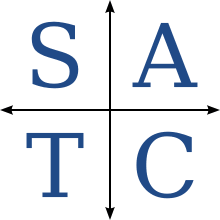
\includegraphics[width=35mm,scale=0.5]{allstudents.png}}

\\[.75in]
\large
Double Angle Formulas

\normalsize
\\~\\
\sin (2\theta) = 2\sin \theta \cos \theta \hspace{10mm}
\cos (2\theta) = \cos^2\theta-\sin^2 \theta
\\~\\
\cos (2\theta) = 1 - 2\sin^2\theta \hspace{10mm}
\cos (2\theta) = 2\cos^2\theta -1

\\[.75in]
\large
Solving Generic Triangles

\normalsize
\\~\\
Heron's Formula: \sqrt{s\cdot(s-a)(s-b)(s-c)}, \hspace{5mm}s=\tfrac{a+b+c}{2}\\[.4in]
Two sides and an included angle: area = \tfrac{1}{2}ab\sin(C)\\[.4in]
\tfrac{\sin(a)}{A}=\tfrac{\sin(b)}{B}




\pagebreak
\Large
Waves

\\[.5in]
\large
Sine
\normalsize
\\~\\

Y=A\sin(Bx+C)+D\\
\\~\\
Amp \Rightarrow \abs A
\\~\\
Period \Rightarrow \dfrac {2\pi }{B}
\\~\\
Phase shift \Rightarrow Bx+C=0, solve for x
\\~\\
Horizontal line of rest \Rightarrow D
\\~\\
Range \Rightarrow [D-\abs{A}, D+\abs{A}]
\\~\\
Domain \Rightarrow (-\infty, \infty)

\\[.75in]
\large
Cosine
\normalsize
\\~\\

Y=A\cos(Bx+C)+D\\
\\~\\
Amp \Rightarrow \abs A
\\~\\
Period \Rightarrow \dfrac {2\pi }{B}
\\~\\
Phase shift \Rightarrow Bx+C=0, solve for x
\\~\\
Horizontal line of rest \Rightarrow D
\\~\\
Range \Rightarrow [D-\abs{A}, D+\abs{A}]
\\~\\
Domain \Rightarrow (-\infty, \infty)

\\[.75in]
\large
Secant
\normalsize
\\~\\

Y=A\sec(Bx+C)+D\\
\\~\\
Amp \Rightarrow None
\\~\\
Period \Rightarrow \dfrac {2\pi }{B}
\\~\\
Phase shift \Rightarrow Bx+C=0, solve for x
\\~\\
Horizontal line of rest \Rightarrow D
\\~\\
Range \Rightarrow (-\infty, D-\abs{A}] \cup [D+\abs{A}, \infty)
\\~\\
Domain \Rightarrow \cos \ne 0
\\(Happens when cosine crosses the HLR and is represented with a v.a.)


\\[.75in]
\large
Cosecant
\normalsize
\\~\\

Y=A\csc(Bx+C)+D\\
\\~\\
Amp \Rightarrow None
\\~\\
Period \Rightarrow \dfrac {2\pi }{B}
\\~\\
Phase shift \Rightarrow Bx+C=0, solve for x
\\~\\
Horizontal line of rest \Rightarrow D
\\~\\
Range \Rightarrow (-\infty, D-\abs{A}] \cup [D+\abs{A}, \infty)
\\~\\
Domain \Rightarrow \sin \ne 0 
\\(Happens when sine crosses the HLR and is represented with a v.a.)




\newpage

\\


\end{center}

\end{document}